\chapter{Major Cavalcanti}

Both the count and Baptistin had told the truth when they announced to
Morcerf the proposed visit of the major, which had served Monte Cristo
as a pretext for declining Albert’s invitation. Seven o’clock had just
struck, and M. Bertuccio, according to the command which had been given
him, had two hours before left for Auteuil, when a cab stopped at the
door, and after depositing its occupant at the gate, immediately
hurried away, as if ashamed of its employment. The visitor was about
fifty-two years of age, dressed in one of the green surtouts,
ornamented with black frogs, which have so long maintained their
popularity all over Europe. He wore trousers of blue cloth, boots
tolerably clean, but not of the brightest polish, and a little too
thick in the soles, buckskin gloves, a hat somewhat resembling in shape
those usually worn by the gendarmes, and a black cravat striped with
white, which, if the proprietor had not worn it of his own free will,
might have passed for a halter, so much did it resemble one. Such was
the picturesque costume of the person who rang at the gate, and
demanded if it was not at No. 30 in the Avenue des Champs-Élysées that
the Count of Monte Cristo lived, and who, being answered by the porter
in the affirmative, entered, closed the gate after him, and began to
ascend the steps.

The small and angular head of this man, his white hair and thick gray
moustaches, caused him to be easily recognized by Baptistin, who had
received an exact description of the expected visitor, and who was
awaiting him in the hall. Therefore, scarcely had the stranger time to
pronounce his name before the count was apprised of his arrival. He was
ushered into a simple and elegant drawing-room, and the count rose to
meet him with a smiling air.

“Ah, my dear sir, you are most welcome; I was expecting you.”

“Indeed,” said the Italian, “was your excellency then aware of my
visit?”

“Yes; I had been told that I should see you today at seven o’clock.”

“Then you have received full information concerning my arrival?”

“Of course.”

“Ah, so much the better, I feared this little precaution might have
been forgotten.”

\begin{figure}[ht]
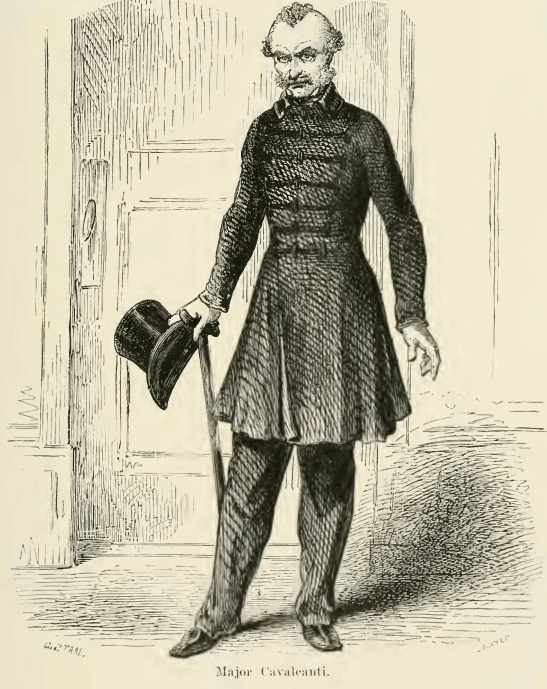
\includegraphics[width=\textwidth]{30119m.jpg}
\end{figure}

“What precaution?”

“That of informing you beforehand of my coming.”

“Oh, no, it has not.”

“But you are sure you are not mistaken.”

“Very sure.”

“It really was I whom your excellency expected at seven o’clock this
evening?”

“I will prove it to you beyond a doubt.”

“Oh, no, never mind that,” said the Italian; “it is not worth the
trouble.”

“Yes, yes,” said Monte Cristo. His visitor appeared slightly uneasy.
“Let me see,” said the count; “are you not the Marquis Bartolomeo
Cavalcanti?”

“Bartolomeo Cavalcanti,” joyfully replied the Italian; “yes, I am
really he.”

“Ex-major in the Austrian service?”

“Was I a major?” timidly asked the old soldier.

“Yes,” said Monte Cristo “you were a major; that is the title the
French give to the post which you filled in Italy.”

“Very good,” said the major, “I do not demand more, you understand——”

“Your visit here today is not of your own suggestion, is it?” said
Monte Cristo.

“No, certainly not.”

“You were sent by some other person?”

“Yes.”

“By the excellent Abbé Busoni?”

“Exactly so,” said the delighted major.

“And you have a letter?”

“Yes, there it is.”

“Give it to me, then.” And Monte Cristo took the letter, which he
opened and read. The major looked at the count with his large staring
eyes, and then took a survey of the apartment, but his gaze almost
immediately reverted to the proprietor of the room.

“Yes, yes, I see. ‘Major Cavalcanti, a worthy patrician of Lucca, a
descendant of the Cavalcanti of Florence,’” continued Monte Cristo,
reading aloud, “‘possessing an income of half a million.’”

Monte Cristo raised his eyes from the paper, and bowed.

“Half a million,” said he, “magnificent!”

“Half a million, is it?” said the major.

“Yes, in so many words; and it must be so, for the abbé knows correctly
the amount of all the largest fortunes in Europe.”

“Be it half a million, then; but on my word of honor, I had no idea
that it was so much.”

“Because you are robbed by your steward. You must make some reformation
in that quarter.”

“You have opened my eyes,” said the Italian gravely; “I will show the
gentlemen the door.”

Monte Cristo resumed the perusal of the letter:

“‘And who only needs one thing more to make him happy.’”

“Yes, indeed but one!” said the major with a sigh.

“‘Which is to recover a lost and adored son.’”

“A lost and adored son!”

“‘Stolen away in his infancy, either by an enemy of his noble family or
by the gypsies.’”

“At the age of five years!” said the major with a deep sigh, and
raising his eye to heaven.

“Unhappy father,” said Monte Cristo. The count continued:

“‘I have given him renewed life and hope, in the assurance that you
have the power of restoring the son whom he has vainly sought for
fifteen years.’”

The major looked at the count with an indescribable expression of
anxiety.

“I have the power of so doing,” said Monte Cristo. The major recovered
his self-possession.

“So, then,” said he, “the letter was true to the end?”

“Did you doubt it, my dear Monsieur Bartolomeo?”

“No, indeed; certainly not; a good man, a man holding religious office,
as does the Abbé Busoni, could not condescend to deceive or play off a
joke; but your excellency has not read all.”

“Ah, true,” said Monte Cristo “there is a postscript.”

“Yes, yes,” repeated the major, “yes—there—is—a— postscript.”

“‘In order to save Major Cavalcanti the trouble of drawing on his
banker, I send him a draft for 2,000 francs to defray his travelling
expenses, and credit on you for the further sum of 48,000 francs, which
you still owe me.’”

The major awaited the conclusion of the postscript, apparently with
great anxiety.

“Very good,” said the count.

“He said ‘very good,’” muttered the major, “then— sir——” replied he.

“Then what?” asked Monte Cristo.

“Then the postscript——”

“Well; what of the postscript?”

“Then the postscript is as favorably received by you as the rest of the
letter?”

“Certainly; the Abbé Busoni and myself have a small account open
between us. I do not remember if it is exactly 48,000 francs, which I
am still owing him, but I dare say we shall not dispute the difference.
You attached great importance, then, to this postscript, my dear
Monsieur Cavalcanti?”

“I must explain to you,” said the major, “that, fully confiding in the
signature of the Abbé Busoni, I had not provided myself with any other
funds; so that if this resource had failed me, I should have found
myself very unpleasantly situated in Paris.”

“Is it possible that a man of your standing should be embarrassed
anywhere?” said Monte Cristo.

“Why, really I know no one,” said the major.

“But then you yourself are known to others?”

“Yes, I am known, so that——”

“Proceed, my dear Monsieur Cavalcanti.”

“So that you will remit to me these 48,000 francs?”

“Certainly, at your first request.” The major’s eyes dilated with
pleasing astonishment. “But sit down,” said Monte Cristo; “really I do
not know what I have been thinking of—I have positively kept you
standing for the last quarter of an hour.”

“Don’t mention it.” The major drew an armchair towards him, and
proceeded to seat himself.

“Now,” said the count, “what will you take—a glass of sherry, port, or
Alicante?”

“Alicante, if you please; it is my favorite wine.”

“I have some that is very good. You will take a biscuit with it, will
you not?”

“Yes, I will take a biscuit, as you are so obliging.”

Monte Cristo rang; Baptistin appeared. The count advanced to meet him.

“Well?” said he in a low voice.

“The young man is here,” said the valet de chambre in the same tone.

“Into what room did you take him?”

“Into the blue drawing-room, according to your excellency’s orders.”

“That’s right; now bring the Alicante and some biscuits.”

Baptistin left the room.

“Really,” said the major, “I am quite ashamed of the trouble I am
giving you.”

“Pray don’t mention such a thing,” said the count. Baptistin re-entered
with glasses, wine, and biscuits. The count filled one glass, but in
the other he only poured a few drops of the ruby-colored liquid. The
bottle was covered with spiders’ webs, and all the other signs which
indicate the age of wine more truly than do wrinkles on a man’s face.
The major made a wise choice; he took the full glass and a biscuit. The
count told Baptistin to leave the plate within reach of his guest, who
began by sipping the Alicante with an expression of great satisfaction,
and then delicately steeped his biscuit in the wine.

\begin{figure}[ht]
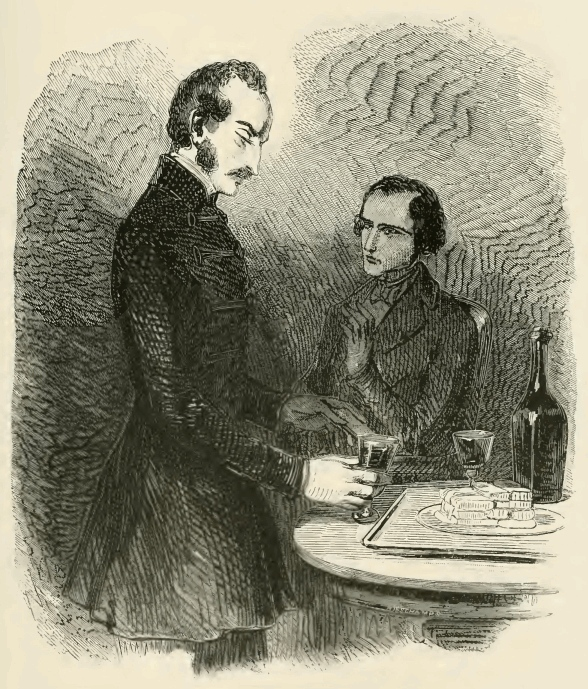
\includegraphics[width=\textwidth]{30123m.jpg}
\end{figure}

“So, sir, you lived at Lucca, did you? You were rich, noble, held in
great esteem—had all that could render a man happy?”

“All,” said the major, hastily swallowing his biscuit, “positively
all.”

“And yet there was one thing wanting in order to complete your
happiness?”

“Only one thing,” said the Italian.

“And that one thing, your lost child.”

“Ah,” said the major, taking a second biscuit, “that consummation of my
happiness was indeed wanting.” The worthy major raised his eyes to
heaven and sighed.

“Let me hear, then,” said the count, “who this deeply regretted son
was; for I always understood you were a bachelor.”

“That was the general opinion, sir,” said the major, “and I——”

“Yes,” replied the count, “and you confirmed the report. A youthful
indiscretion, I suppose, which you were anxious to conceal from the
world at large?”

The major recovered himself, and resumed his usual calm manner, at the
same time casting his eyes down, either to give himself time to compose
his countenance, or to assist his imagination, all the while giving an
under-look at the count, the protracted smile on whose lips still
announced the same polite curiosity.

“Yes,” said the major, “I did wish this fault to be hidden from every
eye.”

“Not on your own account, surely,” replied Monte Cristo; “for a man is
above that sort of thing?”

“Oh, no, certainly not on my own account,” said the major with a smile
and a shake of the head.

“But for the sake of the mother?” said the count.

“Yes, for the mother’s sake—his poor mother!” cried the major, taking a
third biscuit.

“Take some more wine, my dear Cavalcanti,” said the count, pouring out
for him a second glass of Alicante; “your emotion has quite overcome
you.”

“His poor mother,” murmured the major, trying to get the lachrymal
gland in operation, so as to moisten the corner of his eye with a false
tear.

“She belonged to one of the first families in Italy, I think, did she
not?”

“She was of a noble family of Fiesole, count.”

“And her name was——”

“Do you desire to know her name——?”

“Oh,” said Monte Cristo “it would be quite superfluous for you to tell
me, for I already know it.”

“The count knows everything,” said the Italian, bowing.

“Oliva Corsinari, was it not?”

“Oliva Corsinari!”

“A marchioness?”

“A marchioness!”

“And you married her at last, notwithstanding the opposition of her
family?”

“Yes, that was the way it ended.”

“And you have doubtless brought all your papers with you?” said Monte
Cristo.

“What papers?”

“The certificate of your marriage with Oliva Corsinari, and the
register of your child’s birth.”

“The register of my child’s birth?”

“The register of the birth of Andrea Cavalcanti—of your son; is not his
name Andrea?”

“I believe so,” said the major.

“What? You believe so?”

“I dare not positively assert it, as he has been lost for so long a
time.”

“Well, then,” said Monte Cristo “you have all the documents with you?”

“Your excellency, I regret to say that, not knowing it was necessary to
come provided with these papers, I neglected to bring them.”

“That is unfortunate,” returned Monte Cristo.

“Were they, then, so necessary?”

“They were indispensable.”

The major passed his hand across his brow. “Ah, \textit{perbacco},
indispensable, were they?”

“Certainly they were; supposing there were to be doubts raised as to
the validity of your marriage or the legitimacy of your child?”

“True,” said the major, “there might be doubts raised.”

“In that case your son would be very unpleasantly situated.”

“It would be fatal to his interests.”

“It might cause him to fail in some desirable matrimonial alliance.”

“\textit{O peccato!}”

“You must know that in France they are very particular on these points;
it is not sufficient, as in Italy, to go to the priest and say, ‘We
love each other, and want you to marry us.’ Marriage is a civil affair
in France, and in order to marry in an orthodox manner you must have
papers which undeniably establish your identity.”

“That is the misfortune! You see I have not these necessary papers.”

“Fortunately, I have them, though,” said Monte Cristo.

“You?”

“Yes.”

“You have them?”

“I have them.”

“Ah, indeed?” said the major, who, seeing the object of his journey
frustrated by the absence of the papers, feared also that his
forgetfulness might give rise to some difficulty concerning the 48,000
francs—“ah, indeed, that is a fortunate circumstance; yes, that really
is lucky, for it never occurred to me to bring them.”

“I do not at all wonder at it—one cannot think of everything; but,
happily, the Abbé Busoni thought for you.”

“He is an excellent person.”

“He is extremely prudent and thoughtful.”

“He is an admirable man,” said the major; “and he sent them to you?”

“Here they are.”

The major clasped his hands in token of admiration.

“You married Oliva Corsinari in the church of San Paolo del
Monte-Cattini; here is the priest’s certificate.”

“Yes indeed, there it is truly,” said the Italian, looking on with
astonishment.

“And here is Andrea Cavalcanti’s baptismal register, given by the curé
of Saravezza.”

“All quite correct.”

“Take these documents, then; they do not concern me. You will give them
to your son, who will, of course, take great care of them.”

“I should think so, indeed! If he were to lose them——”

“Well, and if he were to lose them?” said Monte Cristo.

“In that case,” replied the major, “it would be necessary to write to
the curé for duplicates, and it would be some time before they could be
obtained.”

“It would be a difficult matter to arrange,” said Monte Cristo.

“Almost an impossibility,” replied the major.

“I am very glad to see that you understand the value of these papers.”

“I regard them as invaluable.”

“Now,” said Monte Cristo “as to the mother of the young man——”

“As to the mother of the young man——” repeated the Italian, with
anxiety.

“As regards the Marchesa Corsinari——”

“Really,” said the major, “difficulties seem to thicken upon us; will
she be wanted in any way?”

“No, sir,” replied Monte Cristo; “besides, has she not——”

“Yes, sir,” said the major, “she has——”

\begin{figure}[ht]
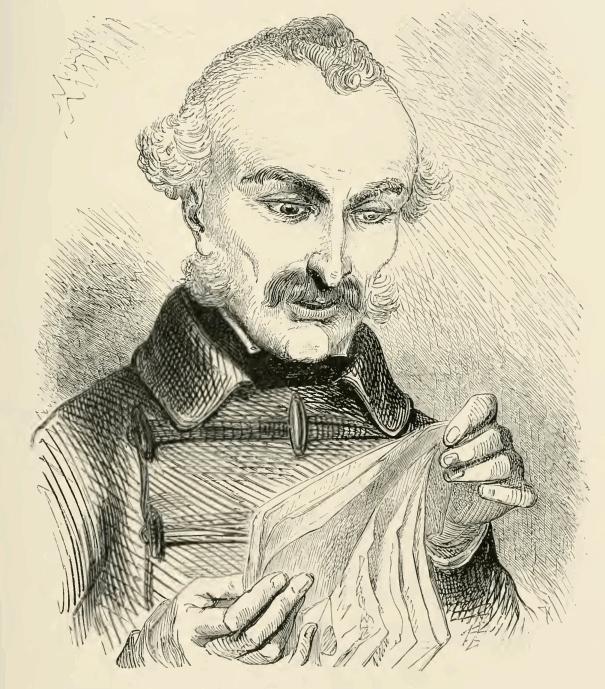
\includegraphics[width=\textwidth]{30127m.jpg}
\end{figure}

“Paid the last debt of nature?”

“Alas, yes,” returned the Italian.

“I knew that,” said Monte Cristo; “she has been dead these ten years.”

“And I am still mourning her loss,” exclaimed the major, drawing from
his pocket a checked handkerchief, and alternately wiping first the
left and then the right eye.

“What would you have?” said Monte Cristo; “we are all mortal. Now, you
understand, my dear Monsieur Cavalcanti, that it is useless for you to
tell people in France that you have been separated from your son for
fifteen years. Stories of gypsies, who steal children, are not at all
in vogue in this part of the world, and would not be believed. You sent
him for his education to a college in one of the provinces, and now you
wish him to complete his education in the Parisian world. That is the
reason which has induced you to leave Via Reggio, where you have lived
since the death of your wife. That will be sufficient.”

“You think so?”

“Certainly.”

“Very well, then.”

“If they should hear of the separation——”

“Ah, yes; what could I say?”

“That an unfaithful tutor, bought over by the enemies of your family——”

“By the Corsinari?”

“Precisely. Had stolen away this child, in order that your name might
become extinct.”

“That is reasonable, since he is an only son.”

“Well, now that all is arranged, do not let these newly awakened
remembrances be forgotten. You have, doubtless, already guessed that I
was preparing a surprise for you?”

“An agreeable one?” asked the Italian.

“Ah, I see the eye of a father is no more to be deceived than his
heart.”

“Hum!” said the major.

“Someone has told you the secret; or, perhaps, you guessed that he was
here.”

“That who was here?”

“Your child—your son—your Andrea!”

“I did guess it,” replied the major with the greatest possible
coolness. “Then he is here?”

“He is,” said Monte Cristo; “when the valet de chambre came in just
now, he told me of his arrival.”

“Ah, very well, very well,” said the major, clutching the buttons of
his coat at each exclamation.

“My dear sir,” said Monte Cristo, “I understand your emotion; you must
have time to recover yourself. I will, in the meantime, go and prepare
the young man for this much-desired interview, for I presume that he is
not less impatient for it than yourself.”

“I should quite imagine that to be the case,” said Cavalcanti.

“Well, in a quarter of an hour he shall be with you.”

“You will bring him, then? You carry your goodness so far as even to
present him to me yourself?”

“No; I do not wish to come between a father and son. Your interview
will be private. But do not be uneasy; even if the powerful voice of
nature should be silent, you cannot well mistake him; he will enter by
this door. He is a fine young man, of fair complexion—a little too
fair, perhaps—pleasing in manners; but you will see and judge for
yourself.”

“By the way,” said the major, “you know I have only the 2,000 francs
which the Abbé Busoni sent me; this sum I have expended upon travelling
expenses, and——”

“And you want money; that is a matter of course, my dear M. Cavalcanti.
Well, here are 8,000 francs on account.”

The major’s eyes sparkled brilliantly.

“It is 40,000 francs which I now owe you,” said Monte Cristo.

“Does your excellency wish for a receipt?” said the major, at the same
time slipping the money into the inner pocket of his coat.

“For what?” said the count.

“I thought you might want it to show the Abbé Busoni.”

“Well, when you receive the remaining 40,000, you shall give me a
receipt in full. Between honest men such excessive precaution is, I
think, quite unnecessary.”

“Yes, so it is, between perfectly upright people.”

“One word more,” said Monte Cristo.

“Say on.”

“You will permit me to make one remark?”

“Certainly; pray do so.”

“Then I should advise you to leave off wearing that style of dress.”

“Indeed,” said the major, regarding himself with an air of complete
satisfaction.

“Yes. It may be worn at Via Reggio; but that costume, however elegant
in itself, has long been out of fashion in Paris.”

“That’s unfortunate.”

“Oh, if you really are attached to your old mode of dress; you can
easily resume it when you leave Paris.”

“But what shall I wear?”

“What you find in your trunks.”

“In my trunks? I have but one portmanteau.”

“I dare say you have nothing else with you. What is the use of boring
one’s self with so many things? Besides an old soldier always likes to
march with as little baggage as possible.”

“That is just the case—precisely so.”

“But you are a man of foresight and prudence, therefore you sent your
luggage on before you. It has arrived at the Hôtel des Princes, Rue de
Richelieu. It is there you are to take up your quarters.”

“Then, in these trunks——”

“I presume you have given orders to your valet de chambre to put in all
you are likely to need,—your plain clothes and your uniform. On grand
occasions you must wear your uniform; that will look very well. Do not
forget your crosses. They still laugh at them in France, and yet always
wear them, for all that.”

“Very well, very well,” said the major, who was in ecstasy at the
attention paid him by the count.

“Now,” said Monte Cristo, “that you have fortified yourself against all
painful excitement, prepare yourself, my dear M. Cavalcanti, to meet
your lost Andrea.”

Saying which Monte Cristo bowed, and disappeared behind the tapestry,
leaving the major fascinated beyond expression with the delightful
reception which he had received at the hands of the count.
